\documentclass[12pt]{article}
\usepackage{fullpage,enumitem,amsmath,amssymb,graphicx}
\usepackage{graphicx} % This is a package for including graphics in your solution.
\usepackage{listings}
\usepackage[final]{pdfpages}

\begin{document}

\begin{center}
{\Large CS168 Spring Assignment 4}

\begin{tabular}{rl}
SUNet ID(s): 05794739 & \\
Name(s): & Luis A. Perez \\
Collaborators: &
\end{tabular}
\end{center}

By turning in this assignment, I agree by the Stanford honor code and declare
that all of this is my own work.

\section*{Part 1}

\begin{enumerate}[label=(\alph*)]
  \item See appendix for code.
  \item
    PCA would recover a uniformly random slope. There is no axis which maximizes the variance of the data, as such the recovered best-fit line would be random.

    LS will recover a line with near 0.0 slope (and y-intercept of 0.5), since this will minimize the distance to the points in the [0,1] x [0,1] square. Any other slope will tend to increase the distance to the opposing corners of the square.

    See code in appendix for simulation.

  \item
    The generated plot is seen in Figure \ref{fig:problem1c}
    \begin{figure}[!ht]
      \centering
      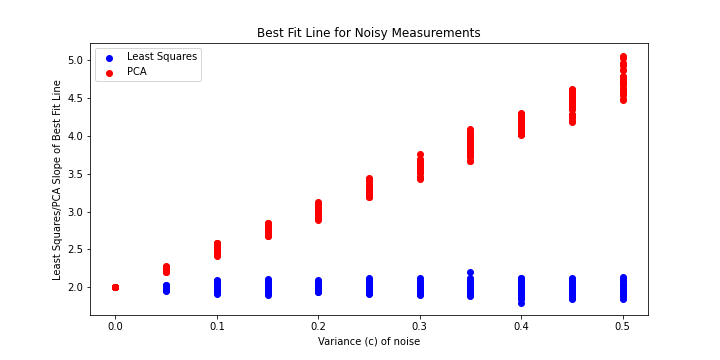
\includegraphics[scale=0.5]{figures/problem1c.png}
      \caption{PCA and Least Squares best-fit line slopes for varying levels of noise in measurement but not input signal. True slope of data is 2.0}
      \label{fig:problem1c}
    \end{figure}

  \item
    The generated plot is seen in Figure \ref{fig:problem1d}
    \begin{figure}[!ht]
      \centering
      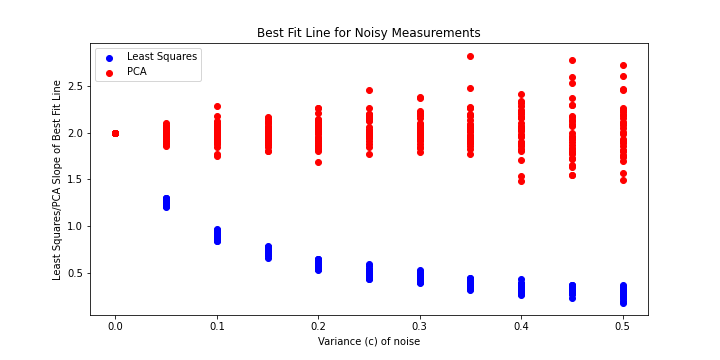
\includegraphics[scale=0.5]{figures/problem1d.png}
      \caption{PCA and Least Squares best-fit line slopes for varying levels of noise in measurement and input signal. True slope of data is 2.0}
      \label{fig:problem1d}
    \end{figure}

  \item
    PCA does poorly when the noise exists only in $Y$ becase it tries to find the direction in which the variability of the data is maximized. By adding noise (additional variability) along the $Y$-axis only, PCA accounts for this by shifting the slop of the line closer to vertical.

    On the other hand, when there's noise along both $X$ and $Y$, the variance along both axis sort of cancels itself out. As such, the principal component will be in the direction of the original slope.

    In this situation where both $X$ and $Y$ are noisy, however, LS will do poorly. Drawing an analogy to our uniformly random points in the unit square, by adding noise along both axes we're approximating a more uniform distribution. As such, the LS solution will begin to favor lines with 0 slope, since this minimizes the distance to all points.

\end{enumerate}

\newpage
\section*{Part 2}

\begin{enumerate}[label=(\alph*)]
  \item
    The dimension would be $10,101$, since this is the number of features.
  \item
    The scatter plot is shown in Figure \ref{fig:pca_genomic_projection}.
    \begin{figure}[!ht]
      \centering
      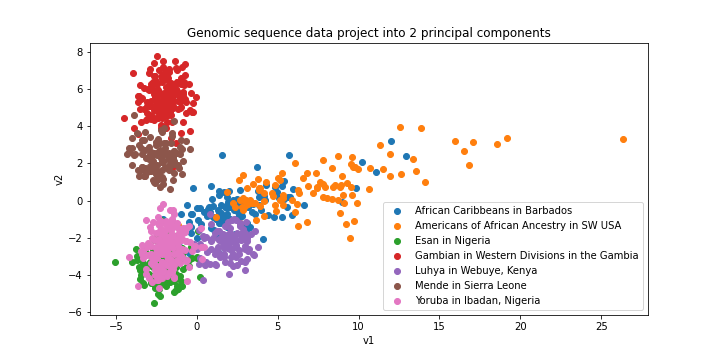
\includegraphics[scale=0.5]{figures/genomic_2d_projection_use_mode=True.png}
      \caption{Genomic data for 995 individuals projected onto the first two principal components as per PCA method.}
      \label{fig:pca_genomic_projection}
    \end{figure}

  \item
    From the plot in Figure \ref{fig:pca_genomic_projection}, we note the following.

    Most populations tends to clusterin groups, with Gambian, Mende, Yoruba, and Esan populations varying primarily along the y-axis, while Luhya, African Caribbeans, and African American's varying the most along the x-axis.

    As such, it appears that $v_1$ (the principal component) has a temporal aspect, since African Caribbeans and African Americans are more recent populations and these vary the most along this axis. It seems to measure the amount of migration. $v_2$ on the other hand appears to capture primarily differences within African-continent populations, so it likely captures more historical/geographical distinctions between these native populations.
  \item
    The scatter plot is shown in Figure \ref{fig:pca_genomic_projection_2}.
    \begin{figure}[!ht]
      \centering
      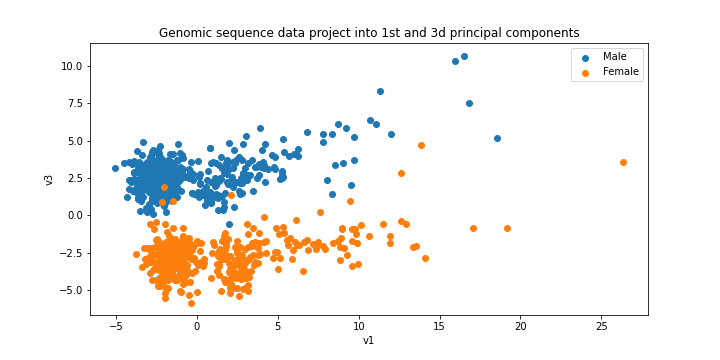
\includegraphics[scale=0.5]{figures/genomic_2d_projection_2.png}
      \caption{Genomic data for 995 individuals projected onto the first and third principal components as per PCA method.}
      \label{fig:pca_genomic_projection_2}
    \end{figure}

  \item
    The third principal component appears to capture gender. 

  \item
    \begin{figure}[!ht]
      \centering
      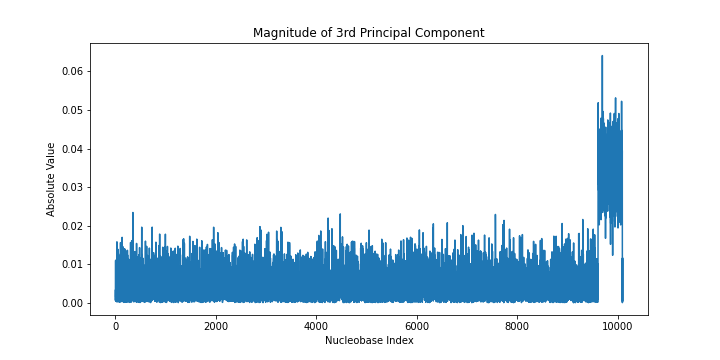
\includegraphics[scale=0.5]{figures/x_y_chromosomes.png}
      \caption{Nucleobase plot of the third principal component which we hypothesized encodes gender.}
      \label{fig:gender_nucleobase}
    \end{figure}
    
    We see the specified plot in Figure \ref{fig:gender_nucleobase}. From this plot, we can see that the last few hundred nucleobases appears to encode information about the Y chromosone, whereas the begining few nucleobases appears to encode information about the X chromosone (larger).

  \item
    We create a bijection by mapping each of $A,T,C,G$ to a one-hot encoded vector. What we mean by this is that our original matrix $X \in \mathbb{R}^{n \times d}$ where $d$ is the feature dimension, would instead become $X' \in \mathbb{R}^{n \times (d x 4)}$ where we conceptually group each of the 4 dimensions to a binary label. 

  \item
    We recreate the plot from (b) above in Figure \ref{fig:projection_full_genome}. We do not see any immediate added value.

    \begin{figure}[!ht]
      \centering
      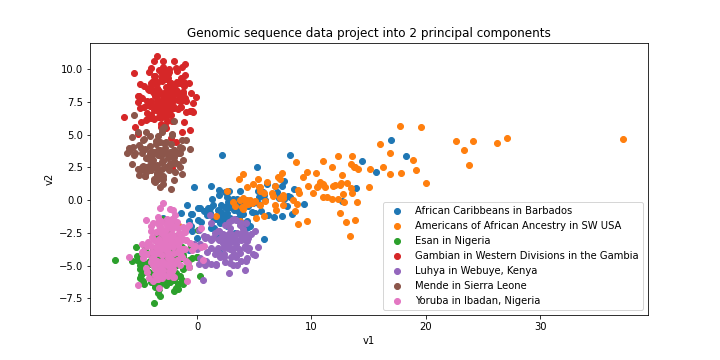
\includegraphics[scale=0.5]{figures/genomic_2d_projection_use_mode=False.png}
      \caption{Genomic data for 995 individuals projected onto the first two principal components as per PCA method with one-hot encoded nucleobases.}
      \label{fig:projection_full_genome}
    \end{figure}

  \item
    It appears that the fourth component capture familiar relationship. We see two cluster along the y-axis in Figure \ref{fig:projection_full_genome_relationship}, where all unrelated individuals are separated into their own own, while individuals from the same family are all clustered together.

    As such, this seems to encode some sense of relatedness to each other in the dataset.

    \begin{figure}[!ht]
      \centering
      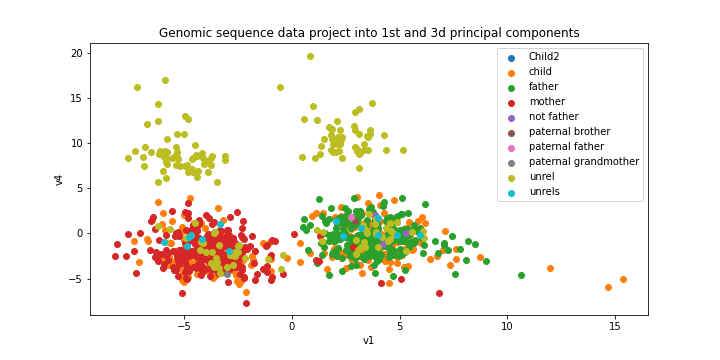
\includegraphics[scale=0.5]{figures/genomic_2i_projection_4th.png}
      \caption{Genomic data for 995 individuals projected onto the third (x-axis) and fourth (y-axis) principal components.}
      \label{fig:projection_full_genome_relationship}
    \end{figure}

  \item NOT DONE.

\end{enumerate}

\newpage
\section*{Appendix}
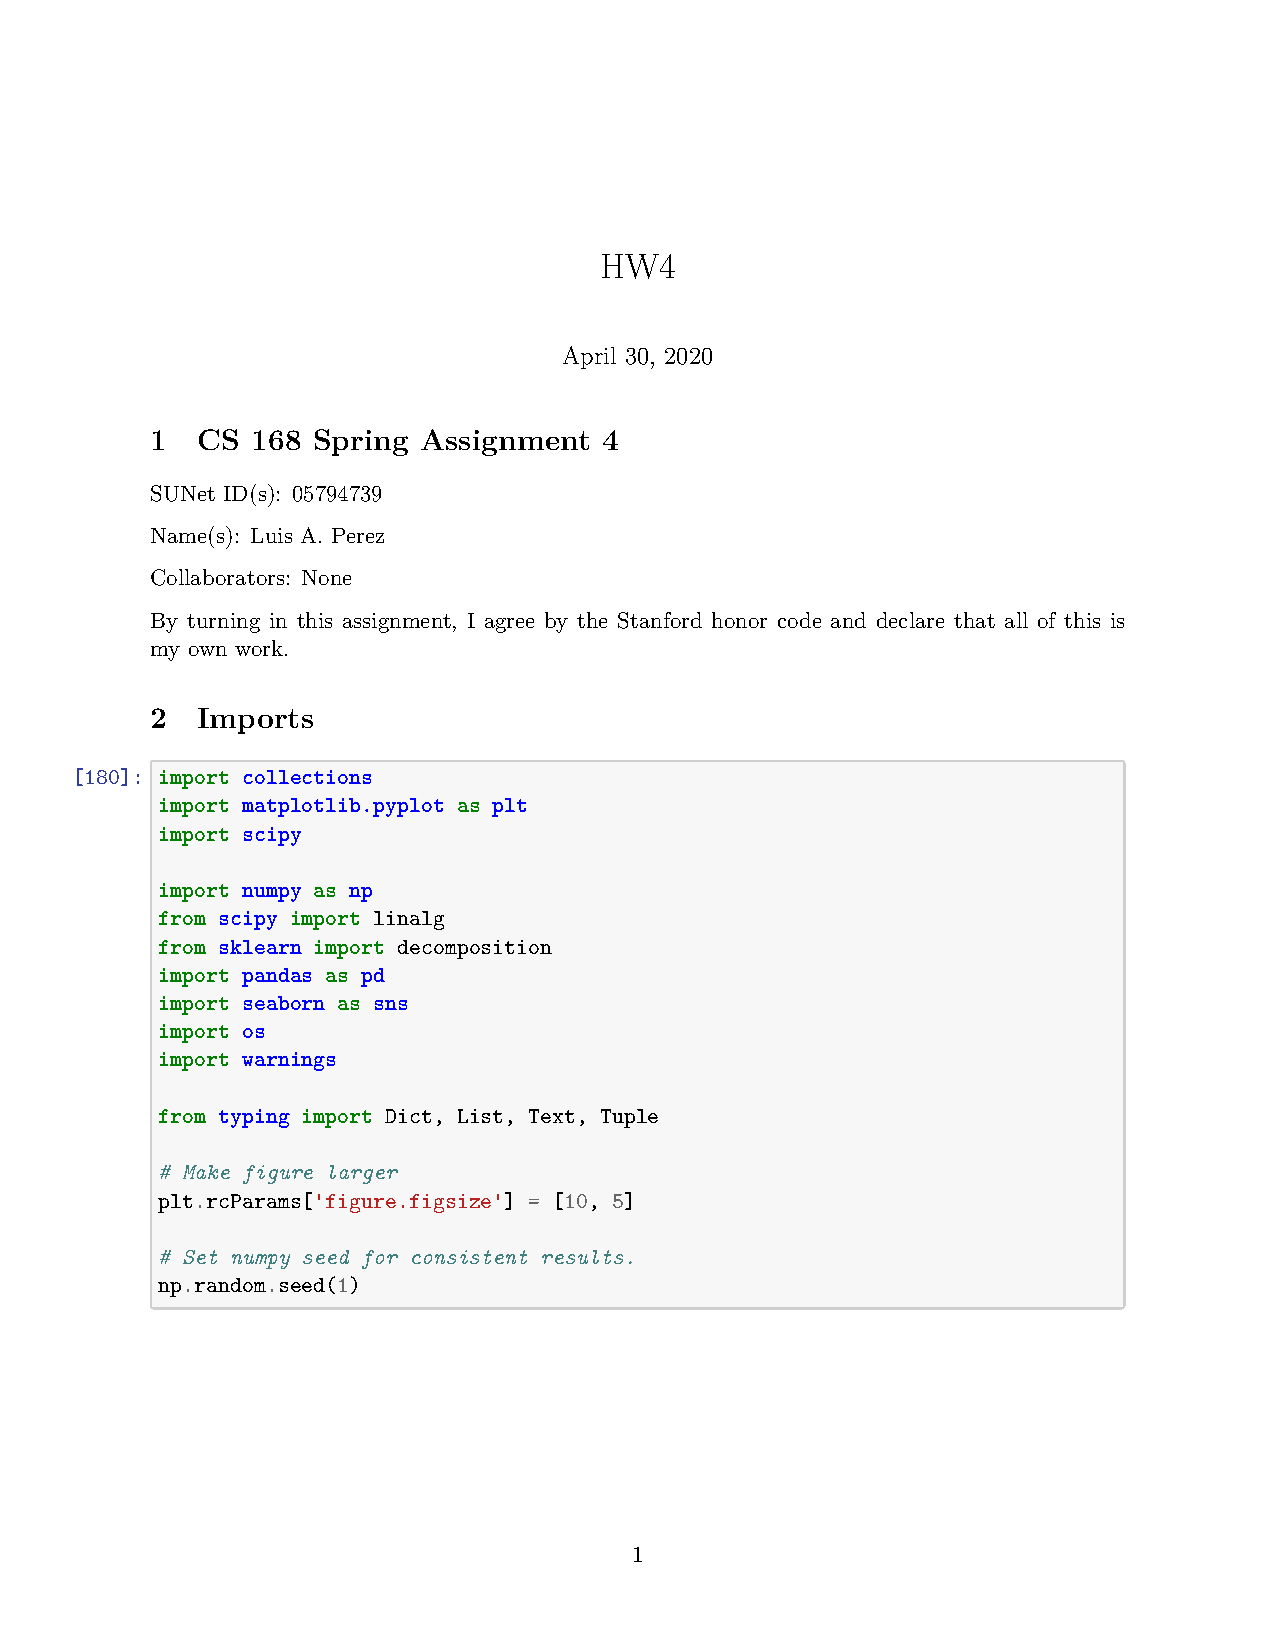
\includepdf[pages=-]{HW4}

\end{document}
